\documentclass{standalone}
\usepackage{pgfplots}
\pgfplotsset{compat=1.17}

\begin{document}
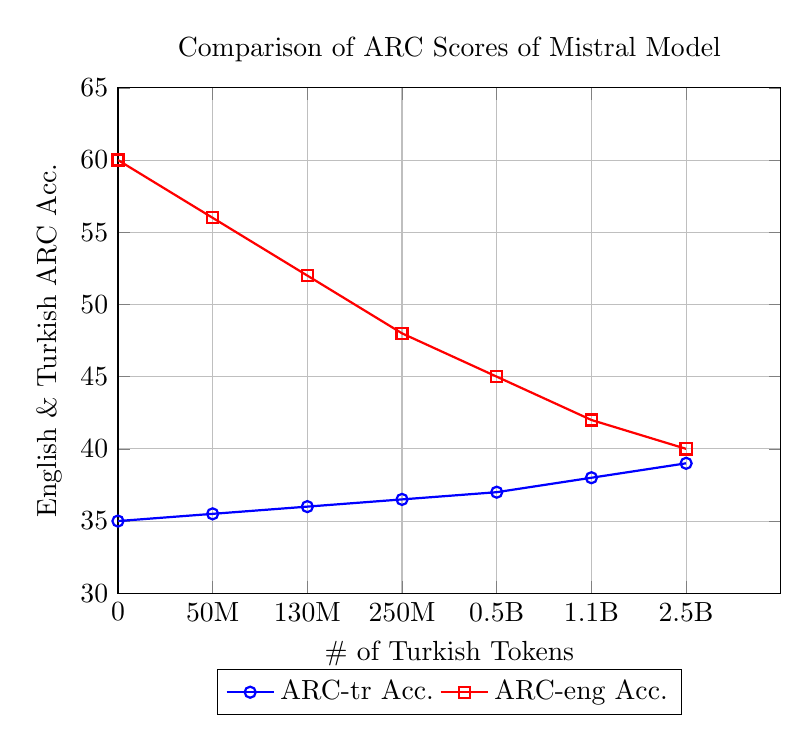
\begin{tikzpicture}
    \begin{axis}[
        width=10cm, height=8cm,
        xlabel={\# of Turkish Tokens},
        ylabel={English \& Turkish ARC Acc.},
        ymin=30, ymax=65,
        xmin=0, xmax=7,
        xtick={0, 1, 2, 3, 4, 5, 6},
        xticklabels={0, 50M, 130M, 250M, 0.5B, 1.1B, 2.5B},
        ytick={30, 35, 40, 45, 50, 55, 60, 65},
        grid=major,
        legend style={at={(0.5,-0.15)}, anchor=north, legend columns=-1},
        legend cell align={left},
        title={Comparison of ARC Scores of Mistral Model}
    ]
    
    % ARC-tr Acc.
    \addplot[
        color=blue,
        mark=o,
        thick
    ]
    coordinates {
        (0,35)(1,35.5)(2,36)(3,36.5)(4,37)(5,38)(6,39)
    };
    \addlegendentry{ARC-tr Acc.}
    
    % ARC-eng Acc.
    \addplot[
        color=red,
        mark=square,
        thick
    ]
    coordinates {
        (0,60)(1,56)(2,52)(3,48)(4,45)(5,42)(6,40)
    };
    \addlegendentry{ARC-eng Acc.}

    \end{axis}
\end{tikzpicture}
\end{document}